
In this chapter the ``detectors' gaps problem'' in Bragg Coherent Diffraction Imaging and our approach to solve it
using Deep Learning are discussed. The main state-of-the-art measures are presented briefly and
the topic of image inpainting with Deep Learning is introduced. The focus will then shift to our works that led
eventually to the optimal ``Patching-based'' approach that can also be found in the published paper entitled
 \textit{``Patching-based deep learning model for the Inpainting of Bragg Coherent Diffraction patterns affected 
 by detectors' gaps''} (\url{https://doi.org/10.1107/S1600576724004163}). The chapter is closed with some analyses 
 of the performances of the DL models in a variety of simulated and experimental cases.  

\section{The ``Gap Problem''}\label{sec:gaps}

At time of writing, standard BCDI experiments employ pixelated photon counting detectors to acquire the diffraction
patterns. These detectors can guarantee high spatial resolution, noise-free counting and fast read-out times. Two examples 
of these devices, currently used at the ID01 beamline are the MAXIPIX and EIGER detectors \cite{ponchut_maxipix_2011, Eiger_Johnson_2014}.
These detectors are often built by tiling together several sensing chips in order to cover a larger area, and are
typically bonded to an Application-Specific Integrated Circuit (ASIC) using bump bonding. 
This implies the presence, in the overall sensing region, of vertical and/or horizontal stripes that are not sensitive
to the impinging radiation. The width of these lines varies depending on the device but normally does not exceed the equivalent 
of some tens of pixels. Specifically, for the MAXIPIX detector the gap size is 6 pixels wide while the EIGER has two types of larger gaps of
12 pixels and 38 pixels width.
The detector gaps problem does not affect BCDI only, but it is shared among other x-ray techniques that deal with single photon-counting
pixelated detectors and/or beamstops.
We have seen in chapter \ref{chp:intro} that during a BCDI scan the 2D images acquired by the detector are stacked to form
a 3D array. This leads these lines to become planes of missing signal in the dataset.
The problems arise when reconstructing the data affected by these gaps. In fact, these regions of non-physical zero intensity
deceive the Phase Retrieval algorithms inducing the presence of artifacts in the reconstructions\cite{carnis_towards_2019}.

\begin{figure}[h]
    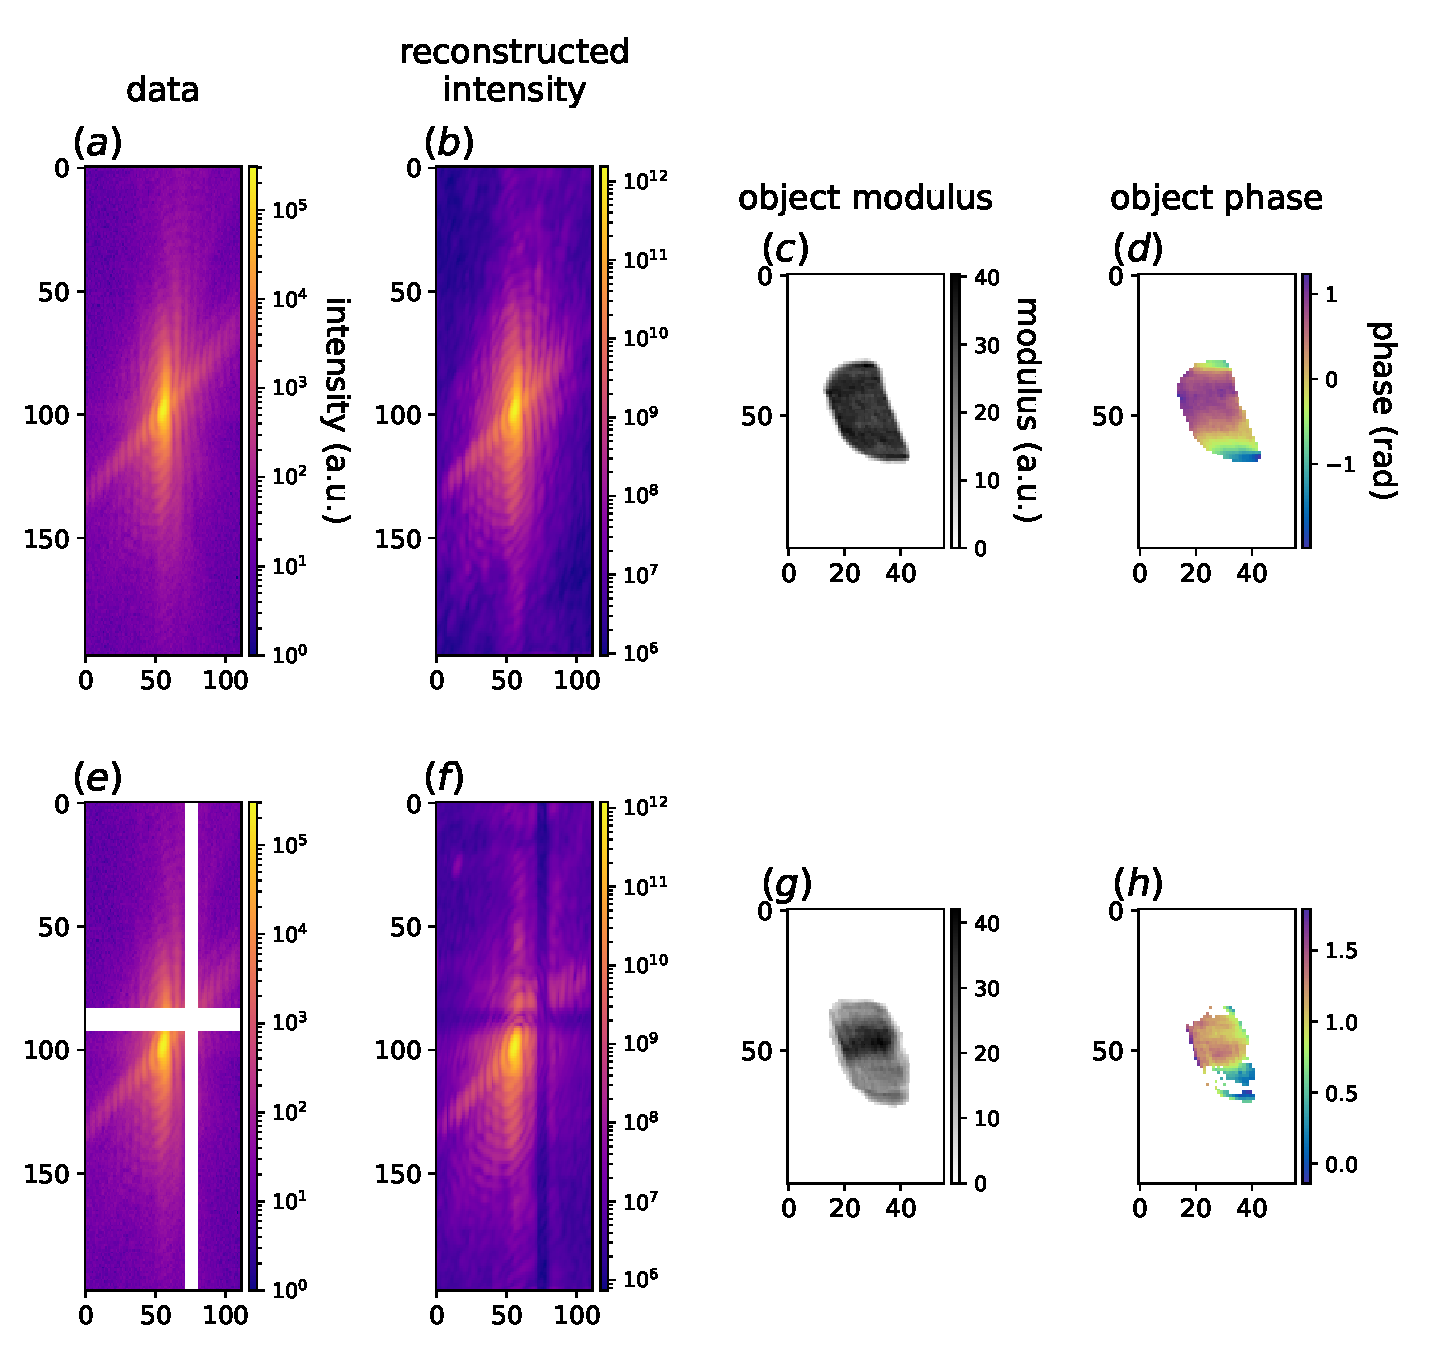
\includegraphics[width=\textwidth]{figures/Inpainting/gaps_intropdf.pdf}
    \caption{\textbf{Effect of detector gaps in BCDI reconstructions} 
    \textbf{(a)} The central xz slice of an experimental diffraction pattern. \textbf{(b)} The same slice of the diffracted
    intensity calculated from the retrieved object. \textbf{(c - d)} xz slice of the modulus and phase respectively of the particle
    obtained from the phasing of the gap-less dataset. \textbf{(e)} Same slice as in \textbf{(a)} with an artificially added
    9 pixel-wide, cross-shaped gaps to mimic the detector's ones. \textbf{(f)} The same slice of the diffracted
    intensity calculated from the retrieved object when not masking the gap regions. \textbf{(h - g)} xz slice of the modulus and phase respectively of the particle
    obtained from the phasing of the gap-affected dataset. The distortions caused by the gaps are evident. }
    \label{fig:gap_intro}
    \end{figure}


It follows that the reliability of the reconstructions in this case is 
compromised as the strain distribution can be deeply affected by the artifacts. A good practice during standard BCDI experiments
is to avoid the gaps by moving the detector if possible. However, this tends to be problematic for the case of high-resolution BCDI, 
i.e. when the diffraction pattern measurement extends to higher q-values, thus covering more than one sensing 
chip and necessarily crossing a gap region. Under these circumstances it becomes important to reduce the amount of
artifacts deriving from the gaps. 


\section{State of the art}\label{sec:InpStateArt}

Here we will discuss the current strategies employed to treat the detector gaps. As someone could argue, the simplest
yet not practical, solution would be to slightly move the detector sideways and acquire a second full scan with the
gap hiding a different region of the same Bragg peak, and then merge the two measurements into a single gap-less one. 
This would more than double the acquisition time making it, de facto, never an option during standard experiments. 

The PyNX software, routinely used for the BCDI phase retrieval at ID01, allows the user to define a mask of the gap 
regions and ignore those pixels during the execution. In this way the quality of the reconstruction improves, 
but one can still notice the presence of high-frequency oscillations appearing in both object's modulus and phase.
The origin of these artifacts can be found in the diffracted intensity calculated from the reconstructed particle as 
one can clearly see that the gap-regions is filled with nonphysically high intensity (see Fig. \ref{fig:gap_intro_mask})

\begin{figure}[h]
    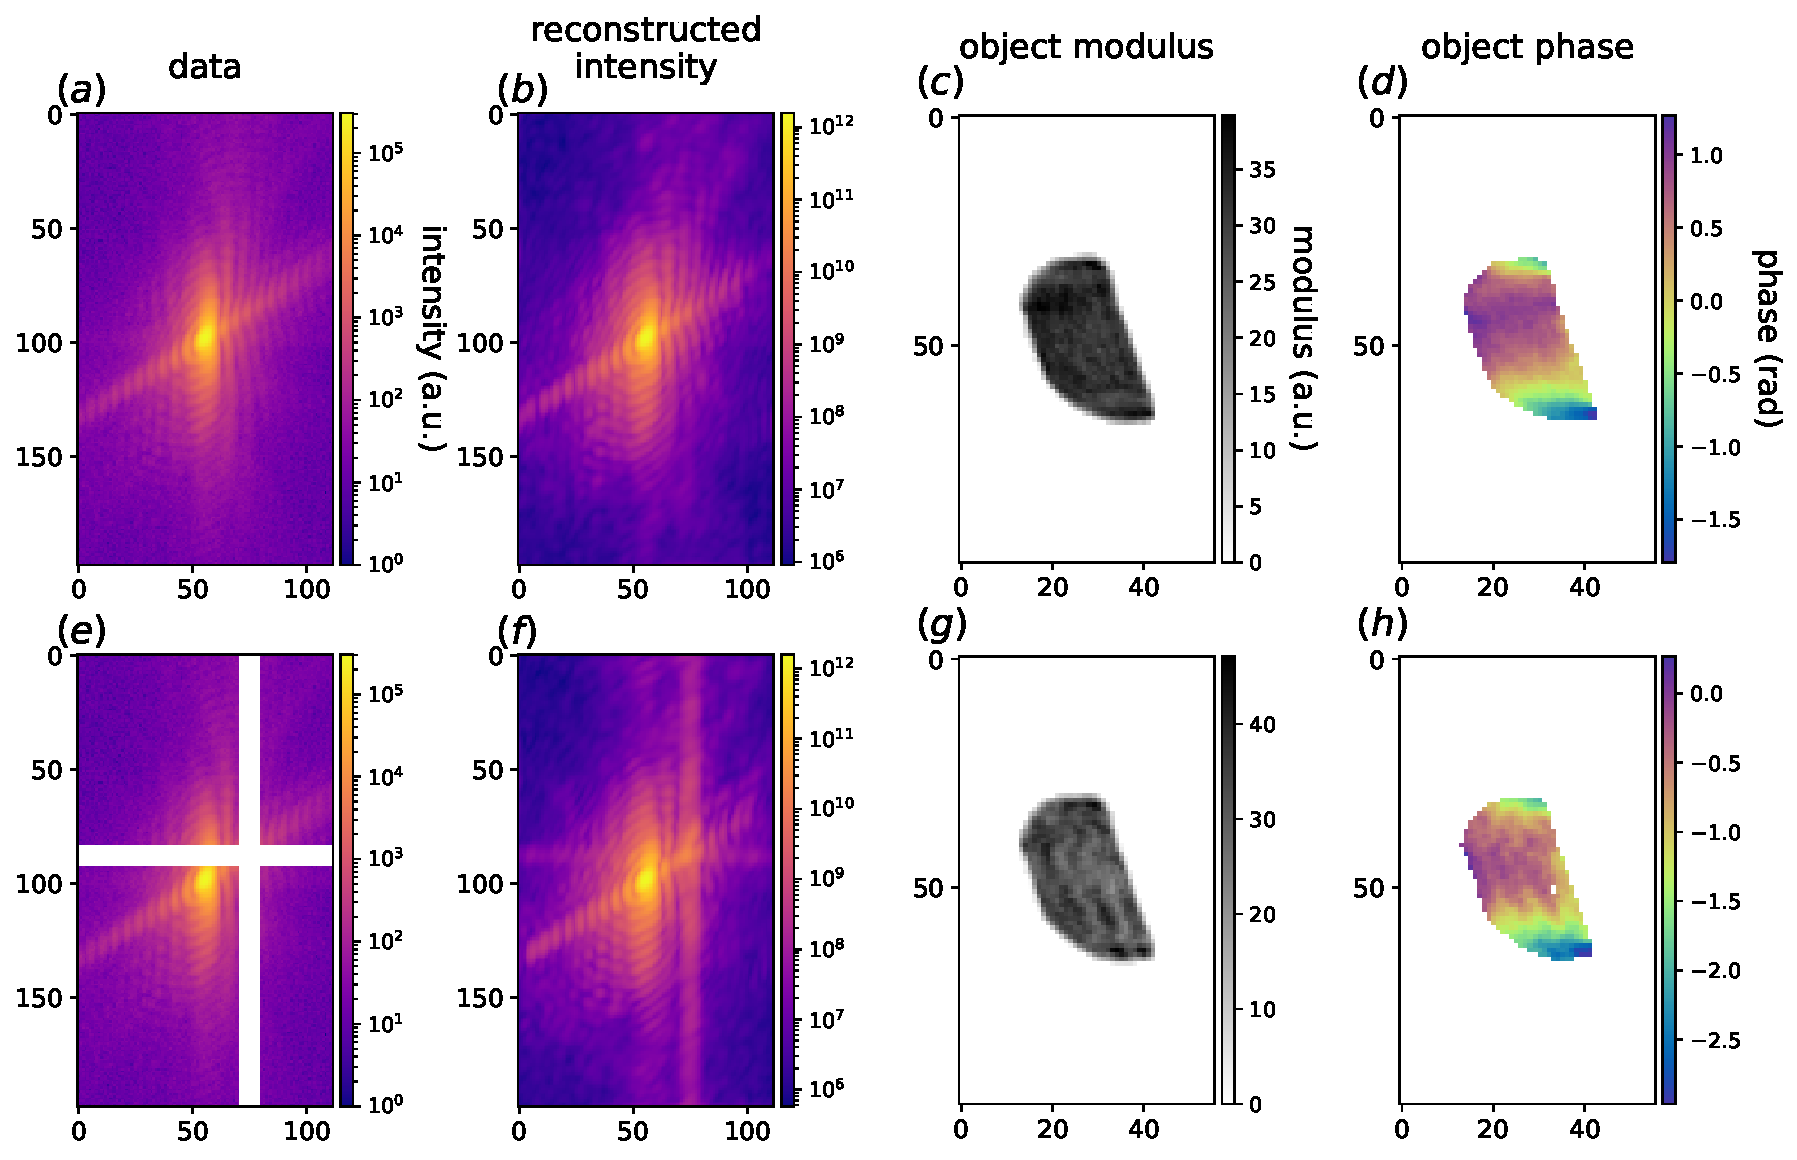
\includegraphics[width=\textwidth]{figures/Inpainting/gaps_mask.pdf}
    \caption{\textbf{Masking the gap region during phasing} 
    \textbf{(a)} The central xz slice of an experimental diffraction pattern. \textbf{(b)} The same slice of the diffracted
    intensity calculated from the retrieved object. Comparing this figure with \ref{fig:gap_intro}\textbf{(b)} one can see that
    when excluding the gap region from the phasing with a mask, the calculated intensity shows bright non-physical streaks 
    instead of the gaps. \textbf{(c - d)} xz slice of the modulus and phase respectively of the particle obtained from the 
    phasing of the gap affected data with a mask of the gap regions. Despite the much higher quality of the reconstruction, 
    one can notice some oscillatory artifacts appearing in both the modulus and the phase of the retrieved object. }
    \label{fig:gap_intro_mask}
    \end{figure}

Another, more invasive, option is to \textit{fill} these gaps with an estimate of the intensity distribution that
would be there, before the phase retrieval. These tasks of filling gap in images is usually referred to as ``inpainting''.
The following paragraph mentions the most relevant inpainting methods to give a context for our work.
    
\subsection{Background on Image Inpainting Research}

 
Computational image inpainting has been widely studied in the field of photography and imaging for many years \cite{Elharrouss_2019,reviewInpainting2021}. 
The inpainting problem can be defined as the task of utilizing known information extractable from the image, to repair
the parts where this information is missing, where for known information the colors, the textures and the semantic features
are intended. In the history of image inpainting a clear cut can be observed when deep learning methods have started to be employed.
For traditional inpainting, different techniques have been explored, from the texture synthesis methods pioneered by Efros and 
Leung \cite{Efros1999} to the use of PDEs as Navier-Stokes equations proposed by Bertalmio \textit{et al.} \cite{BertalmioNavierStokes}
and then again from sparse representations \cite{Mairal_sparse} to hybrid methods combining variational and statistical methods \cite{CedricAllene}

More recently instead, Deep Learning models, headed by Convolutional Neural Networks (CNN), have taken the place of more traditional 
methods as they can attain higher accuracy for more complex inpainting tasks. By undergoing a  
training process, CNNs can ``learn'' to recognize and reproduce the semantic features of the training dataset, and thus
leverage them during inference as additional information beside the colors and textures of the specific image to restore. 
As we have seen in \ref{ch:intro}, the typical CNN architecture for image generation consists of an encoder, which
retains the features of the input image and compresses them into a lower dimensional latent space, and a decoder, which
is responsible for the generation of the output image starting from the latent space. The model are then trained according 
to a loss function that pushes the model's predictions to be close to a given ground truth reference. 
In some cases, the loss function can be replaced by another CNN that is trained to discriminate true images from the ones
predicted by the model. These complementary networks are known as Generative Adversarial Networks (GAN), firstly 
proposed by Goodfellow \textit{et al.} \cite{goodfellow2014generativeadversarialnetworks}, and have also been used for 
image inpainting (e.g. \cite{gan_inpainting}). 
Since reviewing the vast amount of works about CNN for image inpainting is beyond the scope of this thesis and for more 
information, we redirect the reader to the reviews published by Elharrouss \textit{et al.} and Xu \textit{et al.} \cite{reviewInpainting2021,reviewInpaintingDL2023}.
as well as this blog article \cite{towardsdatascience_inpainting}. For what concerns the application of DL based 
inpainting for scientific imaging, early works date back to 2018 as in the case of Sogancioglu \textit{et al.} for x-ray 
human chest 2D radiographic images \cite{sogancioglu2018chestxrayinpaintingdeep} and to 2020 for 2D microscopic images \cite{microscopic_inpainting_2020}.
A couple of years later Tanny Chavez and coauthors published a paper comparing the performances of different CNN models 
for the inpainting of 2D x-ray diffraction images \cite{chavez_comparison_2022}. The work is precisely addressing the 
gap problem for x-ray detectors used for powder diffraction measurements and is awarding UNet and Mixed Scale Dense (MSD) 
models for the best performances on experimental data. The DL models outperform interpolations obtained with biharmonic functions
across 7 and 17 pixel-wide gaps. This work has been of inspiration for the design of our DL model for BCDI gaps inpainting.
In the same year, another work on DL based inpainting for x-ray detector gaps was published by Alfredo Bellisario 
and coauthors \cite{bellisario_noise_2022}. The authors tested a UNet-like model on the inpainting of 2D simulated, noiseless
coherent diffraction patterns against gaps of different sizes (2 to 20 pixels) along the central row. The gaps were 
placed such that the center of the peak was covered, a choice that, as we will see later, yields better results than 
predictions on peripheral areas. To our knowledge, at the time of writing, no other works about deep learning based inpainting
for X-ray detector gaps are present in the literature. \\

\section{Model design: 2D case}\label{sec:model}

On the heels of the last mentioned works we have started to tackle the detector gaps problem for BCDI using CNNs. For simplicity, we started off with 2D
case, using simulated diffraction patterns and inpainting randomly placed vertical gaps of different width. First, we created a training set of 
simulated data, composed of pairs of gap-affected images and corresponding gap-free ground truths, then built a UNet-like model and trained it 
in a supervised fashion.

\subsection{Dataset creation}

The creation of training datasets of simulated 2D BCDI patterns for both the gap-inpainting and phase retrieval tasks has followed the procedure
described in this paragraph.\\
In first place, once chosen the size of the array, a randomly shaped polygon is created in the center using \texttt{scipy.spatial.ConvexHull} 
function. This guarantees the object to have a compact support with homogeneous electron density as assumed for BCDI. Subsequently, 
a random phase field of the same size with variable phase range and correlation length is generated thus the complete complex object is formed.
In order to make the object more realistic a Gaussian filter and Gaussian random noise are applied to the object's modulus, so to smoothen the edges 
and simulate real cases respectively. At this point the object is resized to the shape required to match the chosen oversampling ratio and the 2D
Discrete Fourier Transform is computed. As last stage, Poisson noise is added to the diffraction patterns with different magnitudes to simulate 
various X-ray flux conditions. \\
Datasets contain a number of diffraction patterns in the order of thousands and for each of them the random variables are different as well as the 
oversampling ratios. In the datasets for the training of phase retrieval models, the reciprocal space phase corresponding to each diffraction pattern
is saved as well and used as ground truth label. 
For inpainting tasks a randomly located vertical gap mask was created and applied to the intensity data. In some cases cross-shaped gaps were 
added instead to simulate the experimental condition of the Bragg peak in the vicinity of the corner of the sensing area. 
The size of the gaps was chosen to be consistent across the dataset and four different cases were studied (3px, 6px, 9px, 12px).

\begin{figure}[h]
    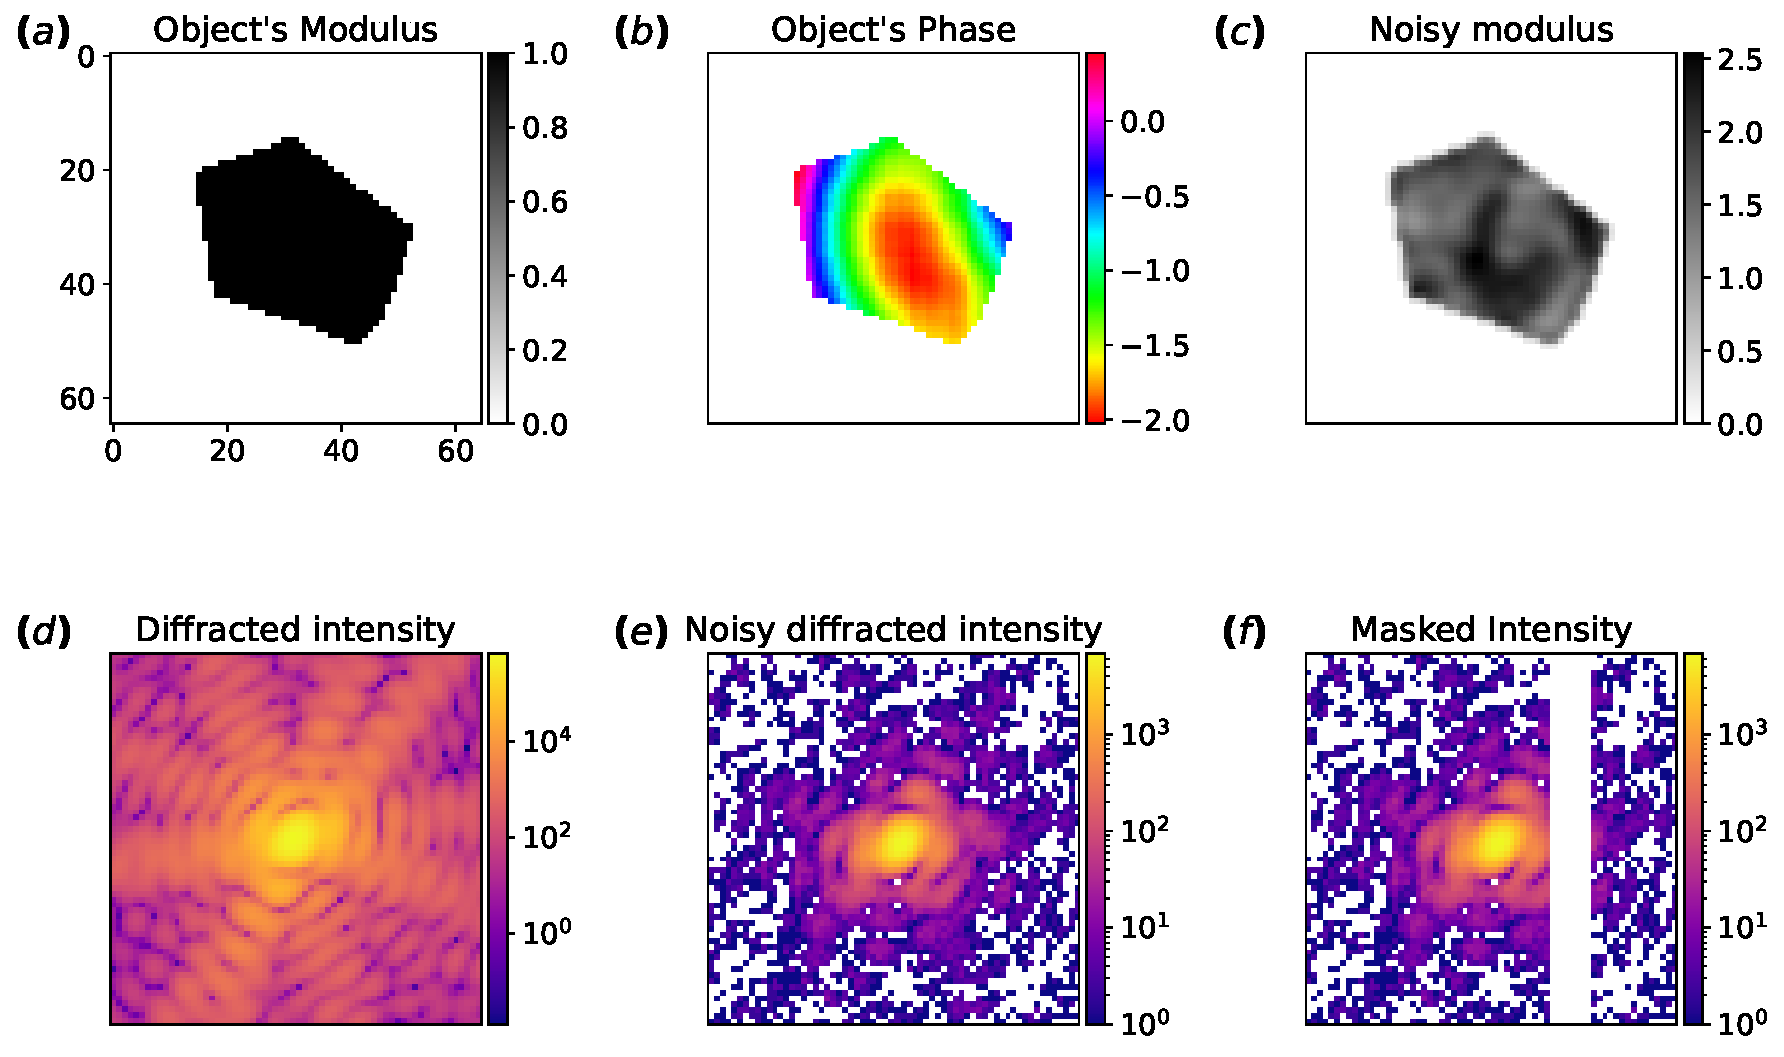
\includegraphics[width=\textwidth]{figures/Inpainting/2D_dataset_creation.pdf}
    \caption{\textbf{Steps for the simulation of a single 2D diffraction pattern} 
    \textbf{(a)} Simulated modulus of a 2D object with random shape and compact support. \textbf{(b)} Simulated object's phase
    \textbf{(c)} Object's modulus after smoothening the edges and adding random Gaussian noise. \textbf{(d)} Squared modulus of the Fourier Transform
    of the complex object (in log scale). The object is first padded with zeros to match the chosen oversampling ratio.
    \textbf{(e)} Poisson noise is added to the simulated diffracted intensity. \textbf{(f)} A 6 pixel-wide
    vertical gap is added to the diffracted intensity at a random position.}
    \label{fig:2D_dataset_creation}
\end{figure}


\subsection{2D Model design}

The 2D model that we have implemented is a UNet that takes in input batches of 32 simulated BCDI patterns affected by vertical and cross-shaped 
gaps. Each diffraction pattern is transformed into logarithmic scale to enhance the features and then normalized between 0 and 1 as convenes to 
every DL model \cite{efficientBackProp}. The shape of each image was chosen to be of $128\times128$ pixels. 
The inputs go through five convolutional blocks inside each of which a convolutional layer, a Leaky ReLU activation
function and a MaxPooling operation are applied. Copies of the output after each convolutional block are sent 
through skip connections to the convolutional blocks of the decoder which concatenate them to the current 
feature tensor. In this way the information flows between encoder and decoder.

\section{Patching approach}\label{sec:patching}
\section{Results in detector space}\label{sec:res_rec}
\section{Results in real space}\label{sec:res_real}
\section{Fine-tuning}\label{sec:finetuning}
\section{Performances assessment}\label{sec:performances}
